\documentclass[12pt,a4]{article} %[font size, tamano de hoja]{Tipo de documento}

\usepackage[left=1.8cm,right=1.8cm,top=32mm,columnsep=20pt]{geometry}

\usepackage[utf8]{inputenc} %Formato de codificación
\usepackage[spanish, es-tabla, es-nodecimaldot]{babel}
\usepackage{amsmath} %paquete para escribir ecuaciones matemáticas
\usepackage{float} %Para posicionar figuras
\usepackage{graphicx} %Para poder poner figuras
\usepackage{hyperref} %Permite usar hipervínculos 
\usepackage{multicol} %Para hacer doble columna
\usepackage[sorting=none]{biblatex} %Imports biblatex package. To cite use \cite{reference_label}
\addbibresource{main.bib} %Import the bibliography file



\title{Métodos Numéricos y Optimización\\

 Trabajo práctico N$^{\circ}$1\\
\vspace{20mm}

 Interpolación y búsqueda de raíces
}

\author{Valentino Arbelaiz y Alejo Zimmermann\\ [2mm] %\\ para nueva línea
\small Universidad de San Andres, Buenos Aires, Argentina}
\date{1er Semestre 2024}
% Tamanos de letra: 
% \tiny	
% \scriptsize
% \footnotesize
% \small	
% \normalsize	
% \large	
% \Large	
% \LARGE	
% \huge	
% \Huge


%Todo lo que está antes de begin{document} es el preámbulo
\begin{document}
\vspace{1cm} % Ajusta la distancia vertical entre la fecha y la imagen



\maketitle
% \begin{center}
% \includegraphics[width=5cm]{logoUdesa.png} % Ajusta la ruta y el tamaño de la imagen
% \end{center}


\begin{abstract}
    Este trabajo estudia el efecto de la distribución de puntos de interpolación en esquemas numéricos de aproximación de funciones uni y bidimensionales, proponiendo una regla para puntos no equiespaciados. Además, se aborda la reconstrucción de trayectorias de vehículos autónomos a partir de mediciones de posición mediante interpolación, determinando el punto de intersección entre dos trayectorias.
\vspace{2mm}
\end{abstract}

\begin{multicols}{2}
\raggedcolumns

\section{Introducción}
En este trabajo se abordan dos problemas generales de los métodos numéricos. Aproximación de funciones y reconstrucción de trayectorias a partir de puntos en un plano.

En la primera parte, se estudiará el efecto que tiene la distribución de los puntos de interpolación en el desempeño de distintos esquemas de interpolación polinómica y spline. Se analizarán funciones unidimensionales y bidimensionales, utilizando inicialmente puntos de colocación equiespaciados. Luego, utilizando los polinomios de Chebyshev para seleccionar puntos de interpolación no equiespaciados y se compararon los resultados obtenidos con los de la distribución equiespaciada estándar.

En la segunda parte, se aplicarán técnicas de interpolación para reconstruir trayectorias de vehículos autónomos en un entorno industrial a partir de mediciones discretas de su posición. Utilizando un conjunto de datos de posiciones GPS registradas, se recuperará la trayectoria de un primer vehículo y se contrastará con la trayectoria real provista. Adicionalmente, se abordará la determinación del punto de intersección entre la trayectoria reconstruida y la de un segundo vehículo a partir de un conjunto más reducido de mediciones de posición.



\section{Métodos}

\textit{A lo largo del trabajo utilizamos los siguientes métodos. }

\subsection{Interpolación}

En la primer seccion de la investigación se estudiaron diversas maneras de interpolación en dos funciones distintas.
\subsubsection{Interpolación de Lagrange}
La Interpolación de Lagrange es un método para encontrar un polinomio que pase por un conjunto dado de puntos. La fórmula para el polinomio interpolante de Lagrange es:

\begin{equation}
    L(x) = \sum_{i=0}^{n} y_i \prod_{j=0, j\neq i}^{n} \frac{x - x_j}{x_i - x_j}
    \label{lagrange}
\end{equation}

Donde $(x_i, y_i)$ son los puntos dados. Este método es útil cuando se tienen pocos puntos y se desea obtener un polinomio que los interpole. Sin embargo, para un gran número de puntos, el polinomio resultante puede oscilar significativamente.
\subsubsection{Interpolación con splines}
El método de interpolación con splines está basado en la interpolación a trozos (piecewise-polynomial interpolation) lo cual consiste en dividir el intervalo principal en subintervalos y realizar una interpolación independiente en cada uno de ellos. La más sencilla es la interpolación lineal a trozos, generando una recta entre cada uno de los nodos. También existe la cuadrática generando funciones cuadráticas en cada subintervalo. Dentro de todos los métodos que existen de interpolación a trozos, en este trabajo se utilizaron los splines cúbicos.

\begin{equation}
    S(x) = a_i + b_i(x - x_i) + c_i(x - x_i)^2 + d_i(x - x_i)^3
    \label{spline cubico}
\end{equation}

Donde $(x_i, y_i)$ son los puntos dados y $a_i$, $b_i$, $c_i$, $d_i$ son los coeficientes del polinomio para el i-ésimo subconjunto. Este método es útil cuando se tienen muchos puntos y se desea obtener una función que los interpole de manera suave, evitando las oscilaciones que pueden ocurrir con la Interpolación de Lagrange.


\subsection{Raíces de Chebyshev}
Los puntos de Chebyshev son un conjunto de puntos utilizados en los métodos numéricos principalmente en la aproximación de funciones. Estos puntos son el conjunto de soluciones de la función de Chebyshev \eqref{Raices Chebyshev}. Pueden generar un impacto en la precisión de las aproximaciones de funciones como durante la interpolación. 
\begin{equation}
    x_{k} = \frac{(a+b)}{2} + \frac{(b-a)}{2} \cos \left( \frac{2k+1}{2n} \pi \right),   
    \label{Raices Chebyshev}
\end{equation}
Con $ k = 0, \ldots, n-1.$ y $n$ es la cantidad de nodos en el intervalo $[a,b]$

\subsection{Búsqueda de raíces}
En la segunda parte, se determinaron las coordenadas en las cuales se cruzan las trayectorias.
\subsubsection{Newton-Raphson}
El método de Newton-Raphson es un método iterativo para encontrar raíces de una función. Se basa en la idea de aproximar la función por una recta tangente en cada iteración y encontrar el punto en el que la recta tangente cruza el eje x. La fórmula de iteración del método de Newton-Raphson es:

\begin{equation}
    x_{n+1} = x_n - \frac{f(x_n)}{f'(x_n)}
\end{equation}

donde $x_n$ es la aproximación en la n-ésima iteración, $f(x_n)$ es el valor de la función en $x_n$, y $f'(x_n)$ es la derivada de la función en $x_n$. El método continúa iterando hasta que se alcanza una tolerancia deseada o se excede el número máximo de iteraciones.


\section{Implementación}

Los métodos previamente presentados se aplicaron a lo largo del proyecto. En la primera sección, se investigó el comportamiento de la interpolación de dos funciones analizadas por separado.
La primer función $f_a(x)$ fue definida mediante la librería NumPy de Python:
\begin{equation}
    f_a (x) = 0.3 ^{|x|}  \cdot \sin(4x) - \tanh(2x) + 2
    \label{$f_a(x)$}
\end{equation}
con $x \in [-4,4]$
\begin{multline*}  
    f_b(x) = 0.75exp\left(-\frac{(10x_1-2)^2}{4}-\frac{(9x_2-2)^2}{4}\right)\\
    +0.65exp\left(-\frac{(9x_1+1)^2}{9}-\frac{(10x_2+1)^2}{2}\right)\\
    +0.55exp\left(-\frac{(9x_1-6)^2}{4}-\frac{(9x_2-2)^3}{4}\right)\\
    -0.01exp\left(-\frac{(9x_1-7)^2}{4}-\frac{(9x_2-3)^2}{4}\right)
\end{multline*}
con $x\in[-1,1]$

Los intervalos fueron divididos en nodos equiespaciados y fueron almacenados en un arreglo de NumPy. Se interpolan las funciones aplicando los métodos mencionados anteriormente utilizando la librería  SciPy. Para la primera función calculamos el error de la interpolación a través de las integrales y comparamos cómo varía el error según los métodos y la cantidad de nodos. También comparamos los errores con puntos no equiespaciados utilizando los nodos de Chebyshev.

En la segunda parte CARLOS ESCRIBI ACA QUE HICISTE

\section{Resultados y análisis}

\textit{En esta sección proponemos figuras, gráficos, tabla comparativas. Todas las tablas y gráficos deben tener rótulos. Las tablas y gráficos deben convencer al lector sobre los resultados obtenidos. En esta sección es donde se logra determinar que método funciona mejor gracias al experimento descripto previamente.}\\
\subsection{Interpolación de funciones }

\begin{figure}[H]
    \centering
    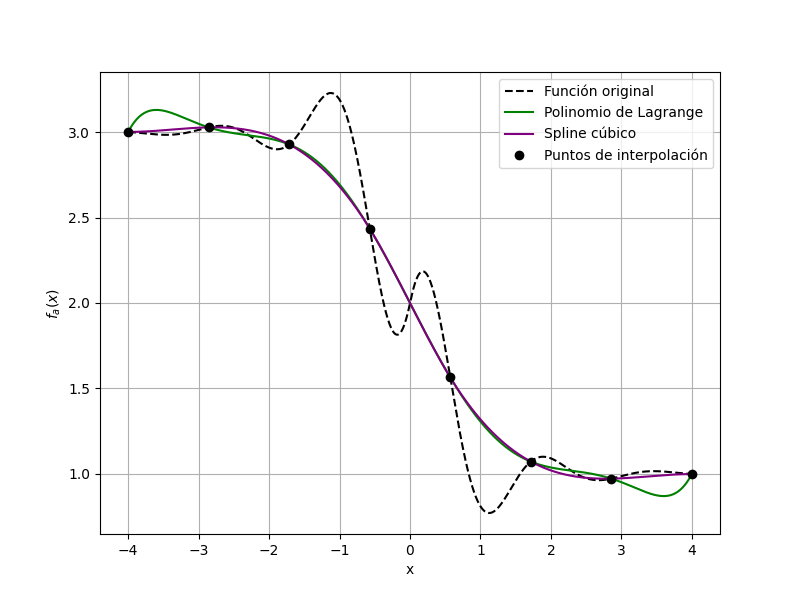
\includegraphics[width=0.8\textwidth]{lagrange_splines_equidistantes.png}
    \caption{Comparación de la interpolación de Lagrange y splines cúbicos}
    \label{fig:lagrange_splines}
\end{figure}

\section{Conclusión}

\textit{En esta sección se hace un resumen de lo realizado en todo el trabajo. Se destacan los descubrimientos mas importantes. Se detallan limitaciones de los métodos. Se pueden incluir futuros pasos. }

Es muy importante tener buenos métodos y el mío es el mejor.

\appendix
\section{Demostración del orden de convergencia del método}
\label{demostracion}

Te la debo.

\printbibliography
\end{multicols}

\end{document}